\graphicspath{{content/chapters/5_Evaluation/figures/}}

\chapter{Evaluation}
\label{chp:evaluation}

\section{Overview}
This chapter evaluates the proof-of-concept system against quantitative ground truth data. Given the exploratory nature of the project, the evaluation focuses on a single representative swim sequence (participant P035, stroke breaststroke, pool length 25.0 m) in which the swimmer completes one full length and returns, yielding a 50 m trajectory. The primary metric is the temporal accuracy with which the system can recover the swimmer's position at known spatial checkpoints. Kinematic outputs, including velocity and wrist-relative motion profiles, are additionally presented and discussed.

\section{Ground Truth Collection}
Ground truth split times were collected retrospectively by reviewing the underwater video footage and manually recording the timestamp at which the swimmer's body cross-ed each 2.5 m marker boundary. This produced 10 outbound checkpoints (2.5 m to 25.0 m) and 10 return checkpoints (22.5 m back to 0.0 m), for a total of 20 reference observations. Times are expressed relative to the detected swim start, defined as the first frame in which sustained forward motion is observed. %!TODO: clarify how the start was defined and detected
All splits were recorded by a single observer, thus no inter-rater reliability measure was applied, which represents an inherent limitation of the ground truth.

\section{Marker Detection Accuracy}
\label{sec:marker_detection}
A foundational element of the positional tracking pipeline is the robust identification of the 2.5 m pool markers. To evaluate the generalisability of the trained object detection model, qualitative assessments were performed comparing its accuracy on the original training video's test split against an unseen video captured in the same pool but under varying environmental conditions.

Figure~\ref{fig:marker_detection_comparison} presents this comparison. The left panels demonstrate the model's performance on test frames extracted from the same sequence used during training. Under these consistent conditions, the model exhibits high confidence and precise bounding box localisation. The right panels depict the model's inference on the unseen sequence. While the physical pool geometry remains identical, differences in ambient lighting, water turbidity, surface glare, and camera positioning introduce a noticeable domain shift. %!TODO: add images to illustrate different env conditions

\begin{figure}[htbp]
    \centering
    \begin{minipage}{0.48\textwidth}
        \centering
        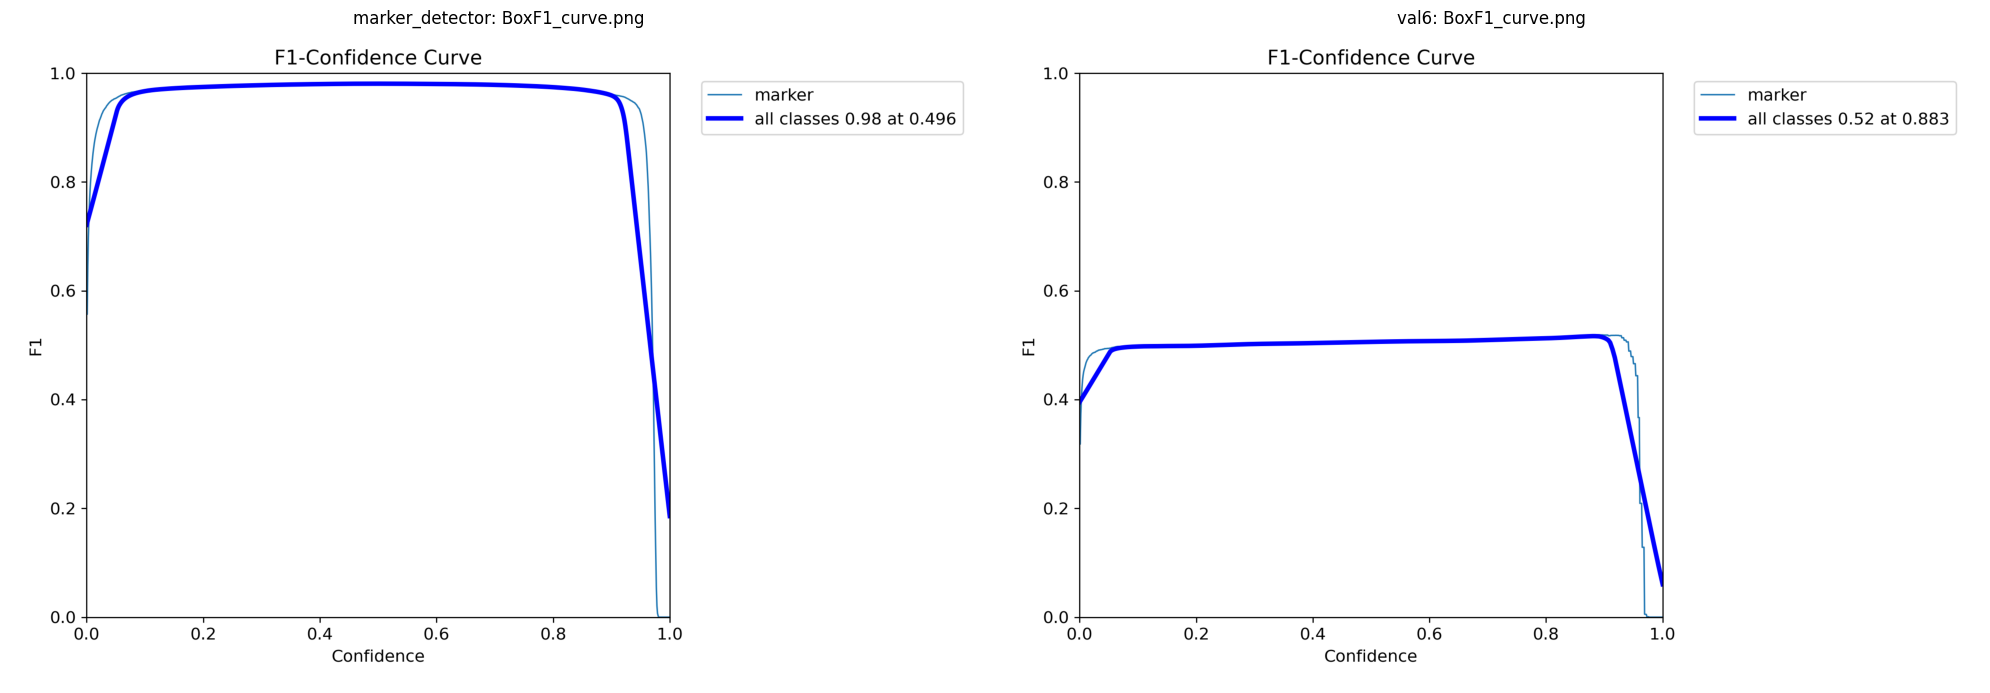
\includegraphics[width=\linewidth]{image_011a7b.png}\\[0.2cm]
        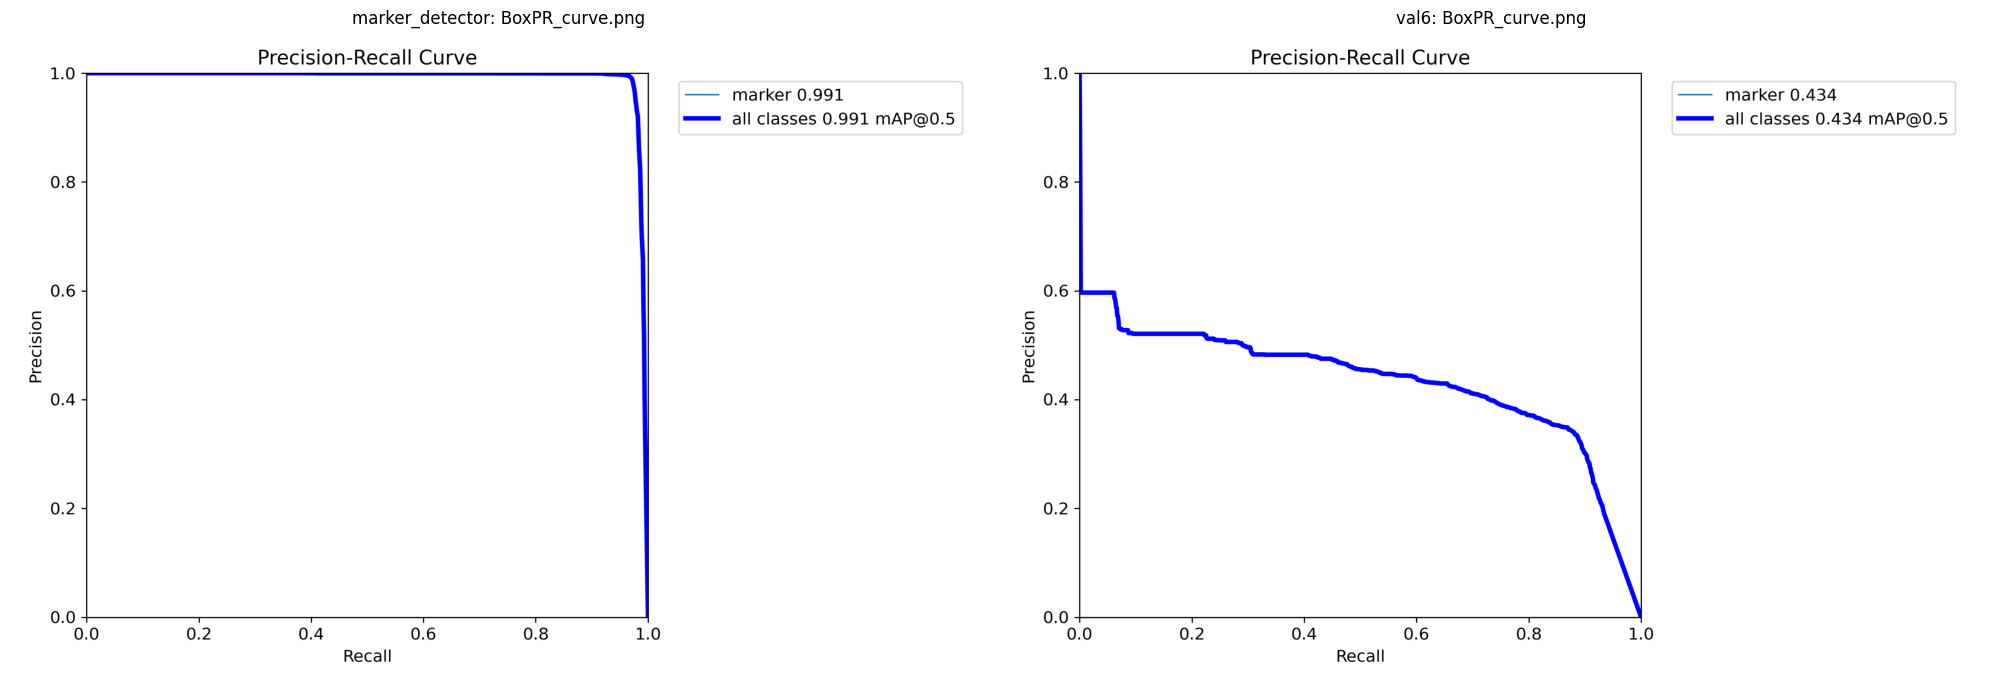
\includegraphics[width=\linewidth]{image_011a60.png}
        \caption*{In-Distribution (Test Frames)}
    \end{minipage}\hfill
    \begin{minipage}{0.48\textwidth}
        \centering
        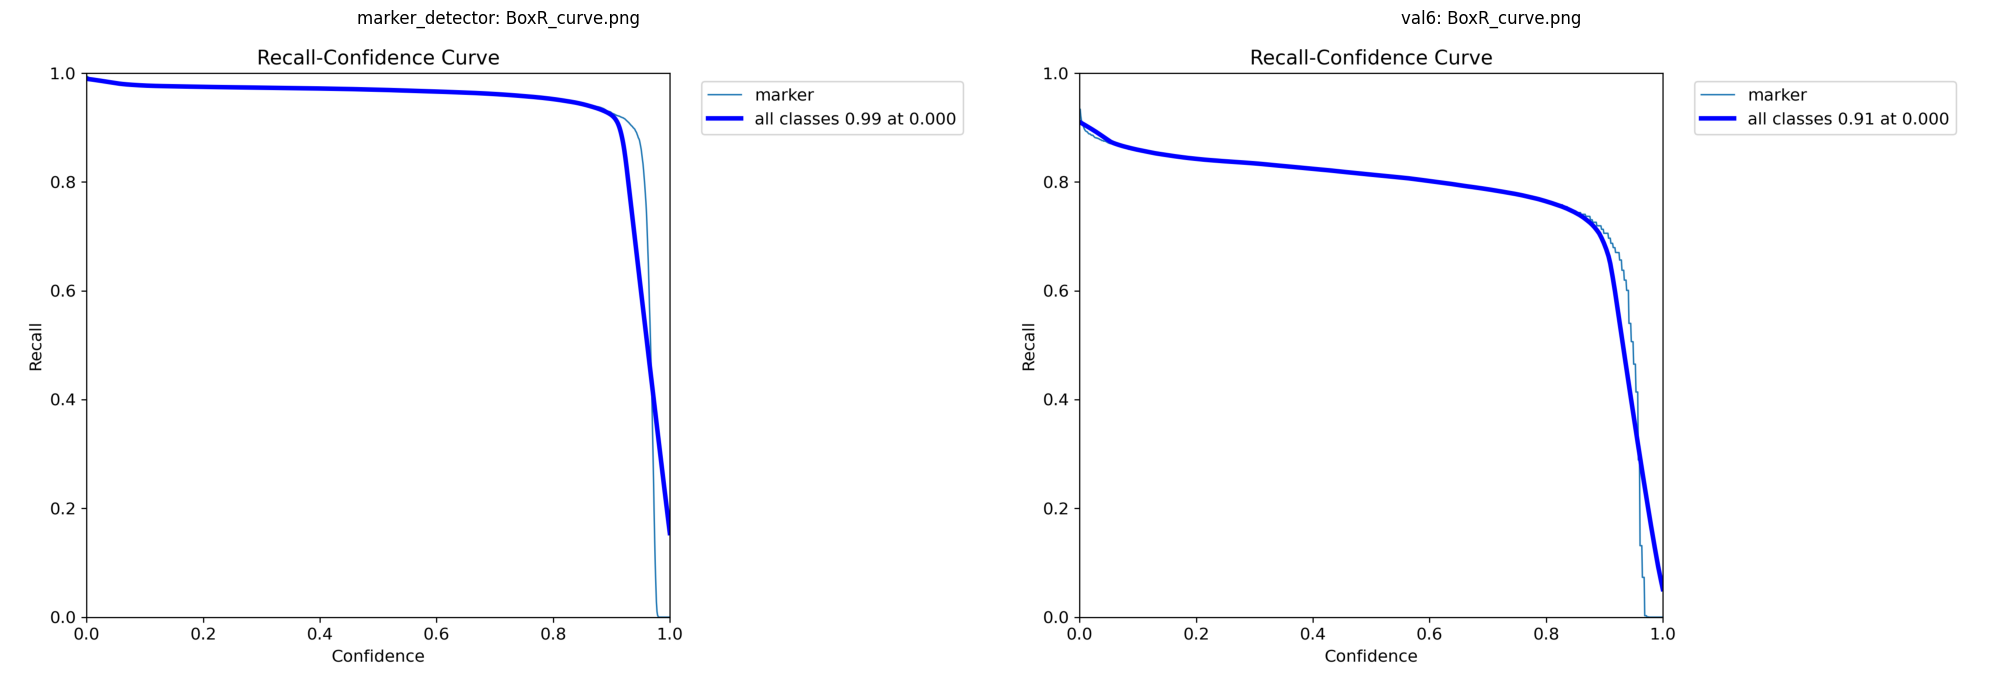
\includegraphics[width=\linewidth]{image_0116a2.png}\\[0.2cm]
        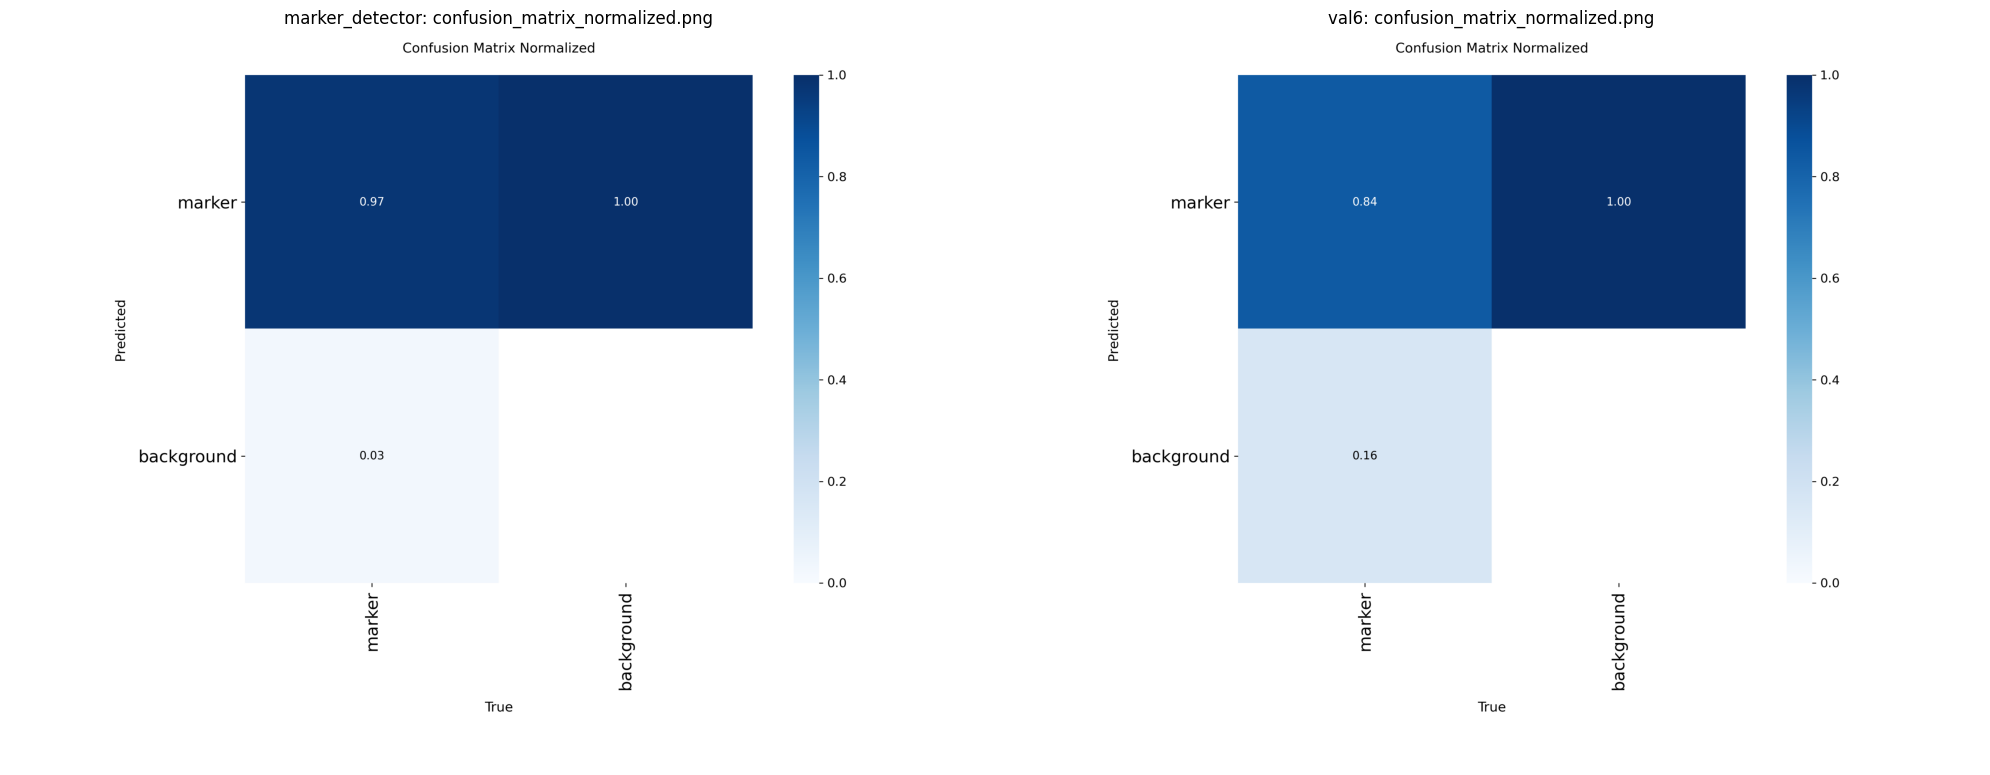
\includegraphics[width=\linewidth]{image_01169b.png}
        \caption*{Out-of-Distribution (Unseen Video)}
    \end{minipage}
    \caption{Comparison of marker detection accuracy. Left: Inference on test frames from the training video, showing high confidence and precision. Right: Inference on an unseen video from the same pool, illustrating the impact of environmental variations such as lighting and turbidity on detection robustness.\label{fig:marker_detection_comparison}}
\end{figure}

Consequently, the model experiences variations in confidence scores and occasional bounding box jitter in the unseen footage. This highlights a common limitation in underwater computer vision: high sensitivity to environmental fluctuations. These variations directly impact the stability of the frame-to-frame pixel-to-metre scale estimation. The subsequent application of the MAD-based inlier filter and Kalman smoothing (discussed in Section~\ref{sec:trajectory_optimisation}) is therefore critical to mitigate these detection inconsistencies and prevent them from propagating as severe positional drift.

\section{Trajectory Optimisation and Pre-Evaluation Processing}
\label{sec:trajectory_optimisation}

\subsection{Outlier Removal}
Prior to evaluation, the raw tracking records were subjected to the MAD-based inlier filter and temporal jump filter described in Chapter~\ref{chp:methodology}. Of the 4,052 raw records, 723 were flagged as significant deviations and removed, leaving 3329 records for downstream processing. A secondary velocity ceiling of 5.0 m/s was subsequently applied, removing a further 32 records whose implied speed was physiologically implausible for competitive breaststroke swimming. %!TODO: add citation for record breaststroke speed and justification why 5m/s 

\subsection{Loop Closure Correction}
The system detects the turn point as the frame index at which the Kalman-filtered position estimate reaches its maximum. For this sequence, the turn was detected at $t = 44.92$ s with a raw maximum position of 27.12 m, requiring an outbound scale correction factor of 0.9218 to anchor the peak exactly at 25.0 m. The return trajectory was subsequently re-mapped using a linear interpolation between the corrected peak and the expected return endpoint. Following loop closure, a Savitzky--Golay filter (window length 61, polynomial order 3) was applied to the centroid velocity signal to suppress residual high-frequency noise.

It should be noted that the two endpoint splits, 25.0 m on the outbound leg and 0.0 m on the return, could not be recovered and are reported as N/A in Table~\ref{tab:split_errors_updated}. The threshold-crossing detection searches for the first frame at which the trajectory strictly exceeds a target distance; because the trajectory is noisy near the turn and near the pool wall, it does not cleanly cross these boundary values, and no valid crossing index is found.

\section{Positional Accuracy Evaluation}

\subsection{Split-Time Comparison}
Table~\ref{tab:split_errors_updated} presents the per-checkpoint comparison between the system's automatically derived split times and the manually recorded ground truth. The error is defined as:
\begin{equation}
    e_i = t_{\text{auto},i} - t_{\text{true},i}
\end{equation}
where a negative value indicates that the system reached checkpoint $i$ earlier than the ground truth observation.

\begin{table}[htbp]
    \centering
    \caption{Updated per-checkpoint split time comparison: automated system vs.\ ground truth. Error $= t_{\text{auto}} - t_{\text{true}}$. (Start at index 385, Turn at index 2041)}
    \label{tab:split_errors_updated}
    \begin{tabular}{llrrr}
        \hline
        Phase                                     & Distance (m)     & True Time (s) & Auto Time (s) & Error (s) \\
        \hline
        Outbound                                  & 2.5              & 2.00          & 2.12          & $+0.12$   \\
        Outbound                                  & 5.0              & 4.00          & 3.88          & $-0.12$   \\
        Outbound                                  & 7.5              & 7.00          & 5.37          & $-1.63$   \\
        Outbound                                  & 10.0             & 9.00          & 8.75          & $-0.25$   \\
        Outbound                                  & 12.5             & 12.00         & 10.15         & $-1.85$   \\
        Outbound                                  & 15.0             & 14.00         & 11.30         & $-2.70$   \\
        Outbound                                  & 17.5             & 17.00         & 16.03         & $-0.97$   \\
        Outbound                                  & 20.0             & 20.00         & 20.50         & $+0.50$   \\
        Outbound                                  & 22.5             & 22.00         & 24.02         & $+2.02$   \\
        Outbound                                  & 25.0             & 26.00         & N/A           & N/A       \\
        \hline
        Return                                    & 22.5             & 27.00         & 28.13         & $+1.13$   \\
        Return                                    & 20.0             & 29.00         & 29.90         & $+0.90$   \\
        Return                                    & 17.5             & 32.00         & 31.37         & $-0.63$   \\
        Return                                    & 15.0             & 35.00         & 33.52         & $-1.48$   \\
        Return                                    & 12.5             & 38.00         & 37.17         & $-0.83$   \\
        Return                                    & 10.0             & 41.00         & 40.07         & $-0.93$   \\
        Return                                    & 7.5              & 43.00         & 42.20         & $-0.80$   \\
        Return                                    & 5.0              & 46.00         & 45.42         & $-0.58$   \\
        Return                                    & 2.5              & 49.00         & 48.37         & $-0.63$   \\
        Return                                    & 0.0              & 51.00         & N/A           & N/A       \\
        \hline
        \multicolumn{4}{l}{\textbf{Overall MAE}}  & \textbf{1.005 s}                                             \\
        \multicolumn{4}{l}{\textbf{Overall RMSE}} & \textbf{1.210 s}                                             \\
        \hline
    \end{tabular}
\end{table}

\subsection{Analysis of Errors}
The system achieves an overall MAE of 1.005 s and an RMSE of 1.210 s across 18 recoverable checkpoints. The error distribution exhibits distinct fluctuations rather than a uniform trend across phases. On the outbound leg, the system initially overestimates swimming speed in the mid-pool section—arriving at checkpoints early and reaching a peak error of $-2.70$ s at the 15.0 m mark. However, this trend reverses towards the end of the lap, where the system underestimates speed and arrives late, generating a $+2.02$ s error at 22.5 m. This suggests non-linear tracking distortions or fluctuating pixel-to-metre scale estimations rather than a simple accumulating drift. On the return leg, errors are slightly smaller in magnitude and more consistent; after initial late arrivals near the turn, the system reliably arrives slightly early, with errors clustering between $-0.58$ s and $-1.48$ s. The full trajectory comparison against ground truth checkpoints is shown in Figure~\ref{fig:trajectory_eval}.

\begin{figure}[htbp]
    \centering
    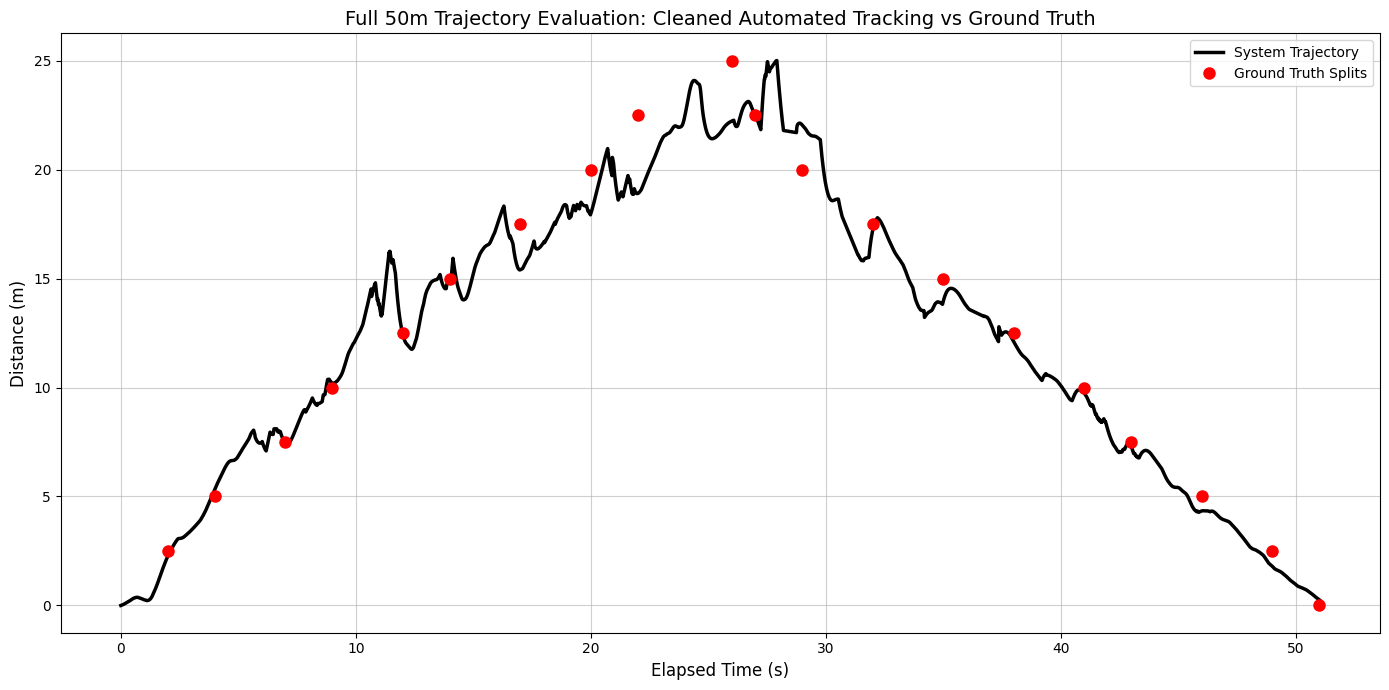
\includegraphics[width=\textwidth]{trajectory_eval.png}
    \caption{Full 50 m trajectory evaluation: system trajectory (black line) versus manually recorded ground truth split times (red points). The swimmer travels from 0 m to 25 m (outbound) and returns to 0 m.\label{fig:trajectory_eval}}
\end{figure}

\section{Kalman Filter Noise Reduction}
As an internal validation of the filtering pipeline, Table~\ref{tab:kalman_noise} reports the standard deviation of the raw and Kalman-smoothed estimates for both position and the pixel-to-metre scale factor. The Kalman filter achieves a modest reduction in position variance and a more substantial reduction in scale variance, reflecting its effectiveness at rejecting the frame-to-frame refractive noise that affects the marker-based scale estimate.

\begin{table}[htbp]
    \centering
    \caption{Raw vs.\ Kalman-filtered standard deviation for position and scale estimates.}
    \label{tab:kalman_noise}
    \begin{tabular}{lrr}
        \hline
        Signal       & Raw $\sigma$ & Kalman $\sigma$ \\
        \hline
        Position (m) & 6.732        & 6.706           \\
        Scale (px/m) & 33.364       & 26.669          \\
        \hline
    \end{tabular}
\end{table}

\section{Kinematic Outputs}

\subsection{Centroid Velocity Profile}
Following loop closure and smoothing, the swimmer's peak speed was estimated at 6.57 m/s (23.65 km/h) and the mean speed at 1.59 m/s (5.73 km/h). These are derived from the Savitzky--Golay smoothed velocity signal rather than the raw Kalman output; the pre-closure Kalman estimate yielded a higher peak of 8.44 m/s, which is physiologically implausible for competitive swimming and reflects residual noise prior to the final smoothing stage. The corrected figures are more consistent with reported competitive breaststroke velocities for recreational to trained swimmers. The full velocity and speed profiles are shown in Figure~\ref{fig:kinematic_profiles}. %!TODO: prob needs some proof for this

\begin{figure}[htbp]
    \centering
    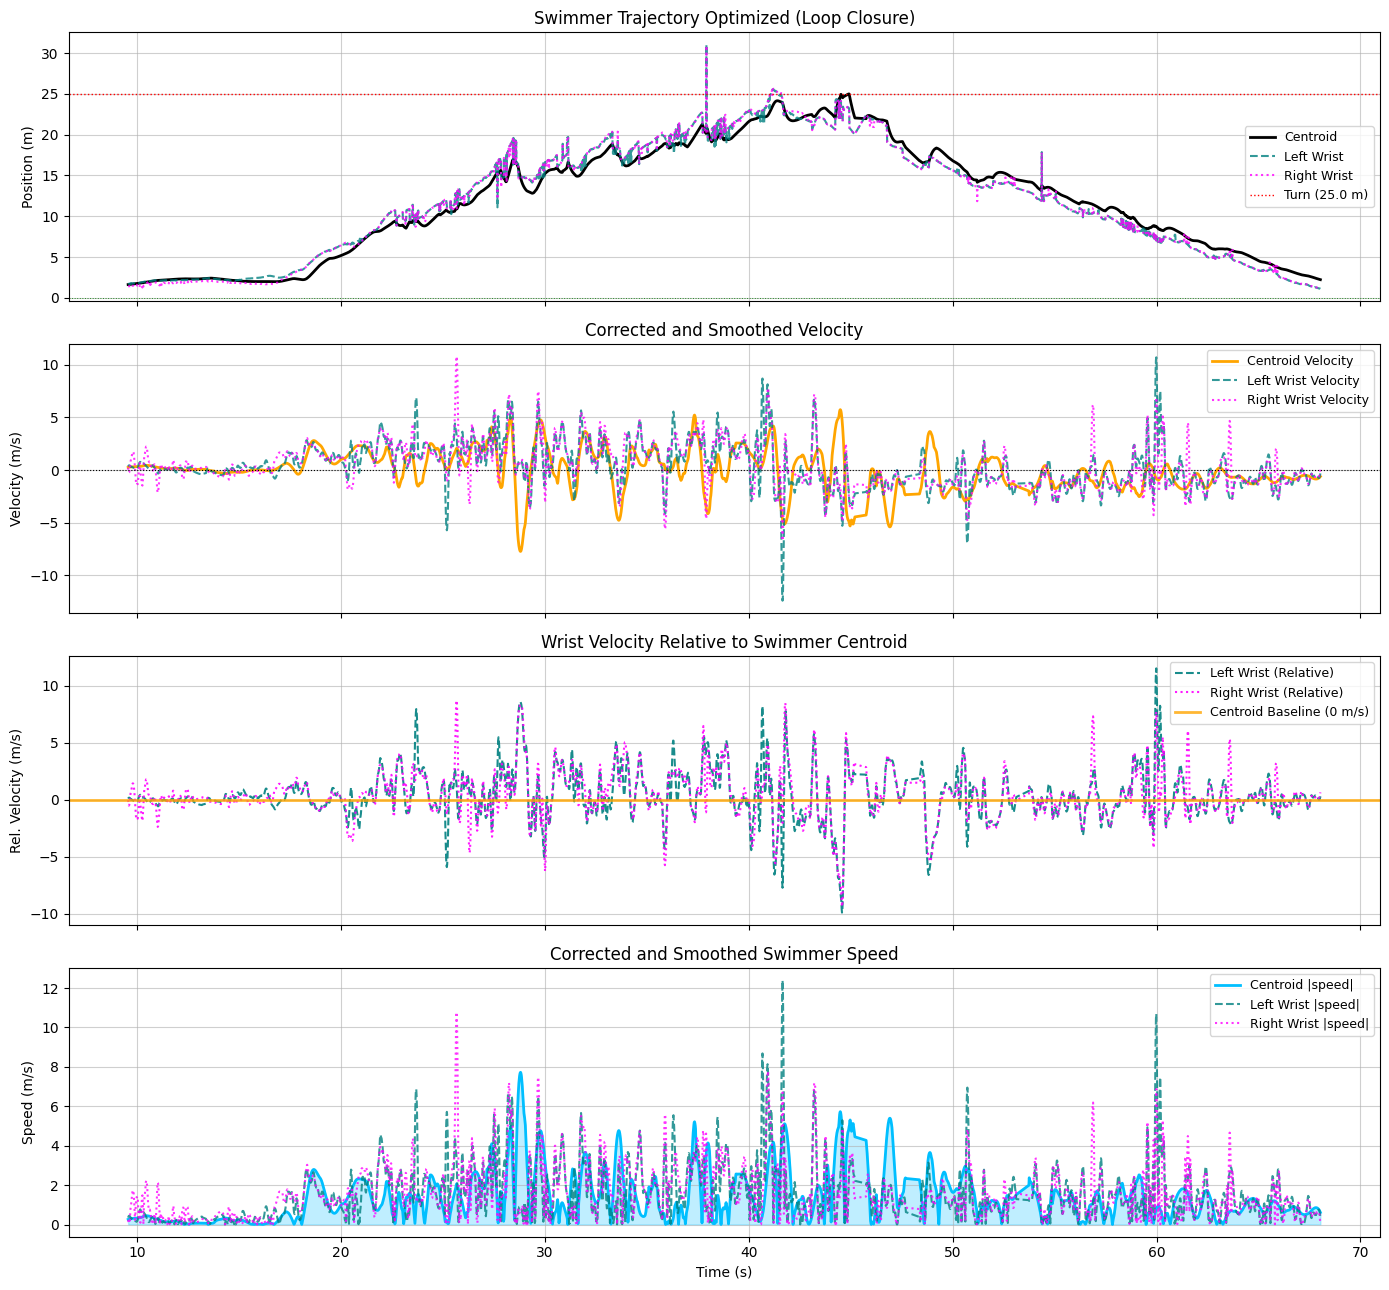
\includegraphics[width=\textwidth]{kinematic_profiles.png}
    \caption{Kinematic profiles for the full 50 m sequence: (top) loop-closure-corrected trajectory for centroid and both wrists; (second) smoothed velocity; (third) wrist velocity relative to swimmer centroid; (bottom) absolute speed magnitude.\label{fig:kinematic_profiles}}
\end{figure}

\subsection{Wrist Kinematics and Symmetry}
To isolate the intra-stroke cycle mechanics from the swimmer's macroscopic forward translation, wrist kinematics were evaluated by subtracting the centroid position from the raw wrist coordinates. This centroid-anchored view is intended to reveal the cyclical pull and recovery phases relative to the swimmer's body. However, as visible in Figure~\ref{fig:kinematic_profiles}, the resulting relative wrist signals exhibit substantial high-frequency noise and spike artefacts throughout the sequence, persisting despite biological thresholding, median filtering, and Savitzky--Golay smoothing. This instability highlights the limitations of the ViTPose keypoint predictions in challenging underwater environments, where partial occlusion, splash, and motion blur frequently cause distal keypoints like the wrists to be dropped or mislocated between frames.

Despite the inherent noise in individual trajectories, evaluating the coordination between limbs provides valuable insights. Because breaststroke dictates simultaneous and symmetrical arm movements, the relationship between the left and right wrists was visualised using a symmetry heatmap (Figure~\ref{fig:wrist_symmetry}). This heatmap plots the spatial correspondence between the two limbs over the duration of the swim. In an ideal stroke with perfect tracking, the distribution would manifest as a highly concentrated, mirrored density.

\begin{figure}[htbp]
    \centering
    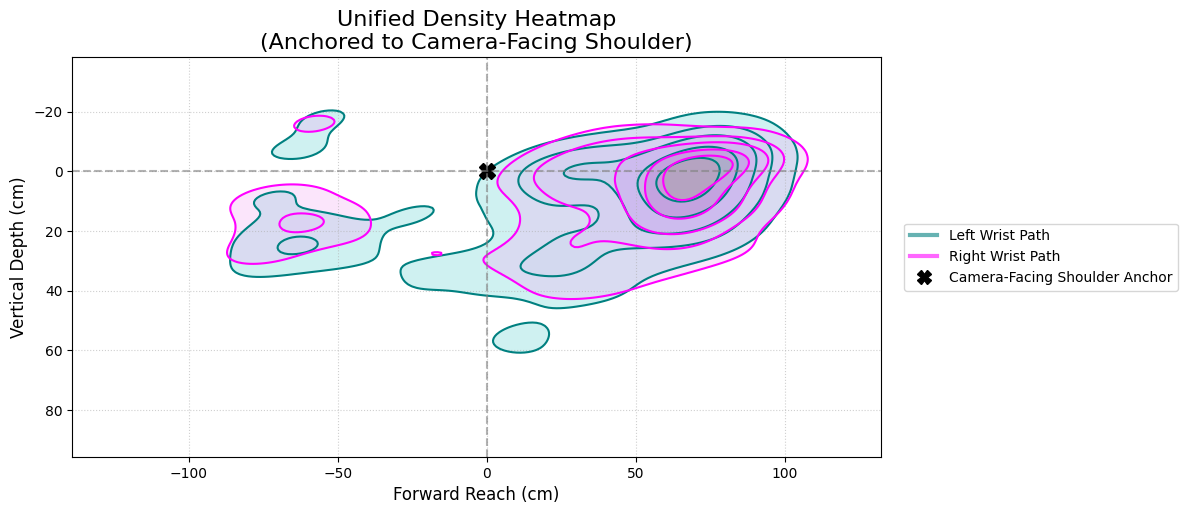
\includegraphics[width=0.8\textwidth]{wrist_symmetry_heatmap.png}
    \caption{Symmetry heatmap illustrating the spatial correlation between the left and right wrist motions relative to the swimmer's centroid. High-density areas indicate the most common spatial relationship between the limbs during the stroke cycle.\label{fig:wrist_symmetry}}
\end{figure}

The generated heatmap exhibits distinct central densities that indicate the underlying stroke rhythm and the overall synchronous nature of the breaststroke pull. However, the presence of asymmetrical dispersion and outliers in the heatmap further corroborates the tracking noise observed in the velocity profiles. While the macro-level phase correspondence between the arms is correctly captured by the model—remaining roughly in phase and appropriately positioned in front of the waist—the fine-grain kinematic noise limits the utility of the current system for precision technique analysis.

\section{Summary}
The system achieves a mean absolute split-time error of 1.005 s and an RMSE of 1.210 s across 18 checkpoints over a 50 m breaststroke sequence, demonstrating that marker-based ego-motion compensation and Kalman filtering can produce a usable positional trajectory from handheld, uncalibrated poolside footage. The primary positional limitation identified is the non-linear fluctuation in scale estimation on the outbound leg—resulting in alternating periods of overestimated and underestimated swimming speed—rather than a strict, continuous monotonic drift. Distal keypoint tracking, particularly for the wrists, remains noisy under water and represents the primary target for future refinement if detailed, centroid-relative technique analysis is desired.